\documentclass[conference]{IEEEtran}
\usepackage{pifont}
\usepackage{times,amsmath,color,tabularx,caption,
amssymb,graphicx,epsfig,cite,psfrag,subfigure,algorithm,multirow,cases,balance}
\newtheorem{claim}{Claim}
\newtheorem{guess}{Conjecture}
\newtheorem{definition}{Definition}
\newtheorem{fact}{Fact}
\newtheorem{assumption}{Assumption}
\newtheorem{theorem}{\underline{Theorem}}
\newtheorem{lemma}{\underline{Lemma}}
\newtheorem{ctheorem}{Corrected Theorem}
\newtheorem{corollary}{\underline{Corollary}}
\newtheorem{proposition}{Proposition}
\newtheorem{example}{\underline{Example}}
\newtheorem{remark}{\underline{Remark}}
\newtheorem{problem}{\underline{Problem}}
\def\Ei{\mathop\mathrm{Ei}}
\def\E{\mathop\mathrm{E}}
\def\tr{\mathop\mathrm{tr}}
\newcounter{mytempeqncnt}
%\IEEEoverridecommandlockouts

\begin{document}

\title{Literature Survey \\ Unsupervised Feature Learning and Deep Learning}
\author{Jiachen Li (Andrew ID: jiachenl)\\%
Language Technologies Institute, Carnegie Mellon University, Pittsburgh, PA, 15213, USA\\
Email: jiachenl@cs.cmu.edu
}

%\thanks{This work was supported...}




\maketitle %\thispagestyle{empty}




\begin{abstract}
Machine Learning has proven to be a big success in many areas of artificial intelligence. However, the success of these algorithms highly depends on how good the features are represented. A good representation of feature is surely
to enhance the performance of machine learning algorithms, while a poor representation may not only severely limit the performance
but even ruin the results. In this literature survey, I will do a review on the field of unsupervised feature learning and has an emphasis on learning feature representation through deep learning architecture. This survey will start with the problems about unsupervised feature learning. After that, it will introduce some typical algorithms in unsupervised feature learning and deep learning. Moreover, it will provide a few successful examples by using unsupervised feature learning. Finally, the limitation, conclusion as well as the potential feature works will be included at last.

\end{abstract}

\section{Introduction}

The performance of machine learning algorithms, especially the simpler ones  highly depends on how good the features are represented \cite{review}. For this reason, much of the effort in deploying machine learning algorithms in real problems has been paid to the process of feature extraction. During the past decades, feature extraction does play an very important role in the development of machine learning, where the machine learning research communities have spent a lot of efforts on manually designing or creating new features through domain knowledge and some other special techniques. For example, the MFCC feature in speech recognition and the HoG feature in computer vision. However, though these features may often contain the deep insights about a specific problem or some incredibly clever ideas, we cannot avoid the fact that the way to create such features costs a lot of human labor and the feature representation derived often cannot be extended to other problems, especially when we encounter into them in a new filed. So the problems that whether there is any way to learn the feature representation automatically and whether there is any way to do better than the manually created features come up. Fortunately, the answer is yes to both of the questions, and the way is unsupervised feature learning.

\subsection{What Is Unsupervised Feature Learning?}

\begin{figure}[t]
\centering
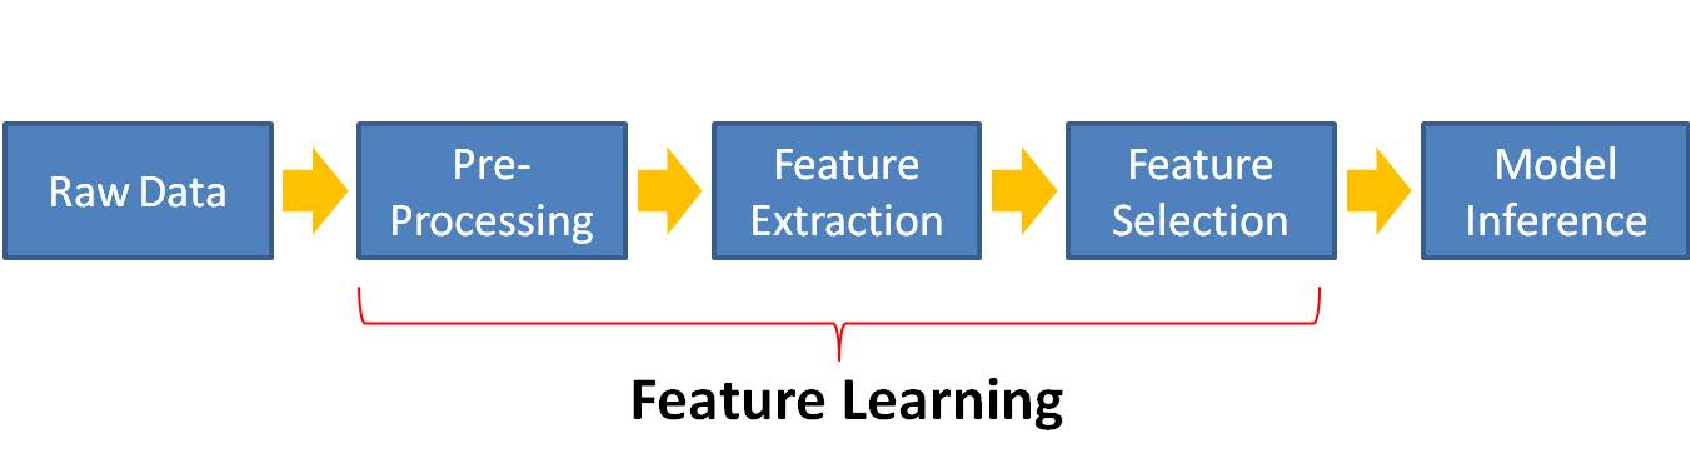
\includegraphics[width=85mm]{feature_learning.pdf}
\caption{The general framework of machine learning task and the definition of feature learning.}
\label{fig:ml_task}
\end{figure}

To answer the question that what is unsupervised feature learning, let's start by looking at the general framework of solving a machine learning task. To solve a machine learning problem, as shown in Fig. \ref{fig:ml_task}, we should first do pre-precessing for the raw data, such as the data cleaning, and then perform feature extraction on the processed data. After that, we apply our feature extraction algorithm to extract the useful features, do feature selection on these extracted features and then use them for training models. With a well trained model, we can finally approach to our goals like classification or regression.

In the above framework, the procedures of pre-processing, feature extraction and feature selection together can be summarized as ``feature learning''.
Moreover, the term ``unsupervised'' means that we want this kind of feature learning procedures to be performed without our supervision (knowledge) or even without any of our help.

\subsection{Differences with other Machine Learning Tasks}



One of the major differences that distinguishes unsupervised feature learning from other machine learning tasks such as classification is the ultimate goal during the training phase. To be specific, in the problem of classification, the typical objective is to minimize the classification errors on the training set, so that we can learn a classifier or predictor for future use. However, in the unsupervised feature learning, the goal changes to learn the representation of feature automatically, which means the algorithms will make their own decisions on what is going to learn. Therefore, the features learned will no long be specified by human, which is totally different from the paradigm of feature engineering where people design by hands on what to learn.

%\subsection{Types of Unsupervised Feature Learning}

%There are two common unsupervised feature learning settings, depending on what type of unlabeled data you have. The more general and powerful setting is the self-taught learning setting, which does not assume that your unlabeled data $\mathbf{x}_u$ has to be drawn from the same distribution as your labeled data $\mathbf{x}_l$ \cite{self_taught}. The more restrictive setting where the unlabeled data comes from exactly the same distribution as the labeled data is sometimes called the semi-supervised learning setting. This distinctions is best explained with an example, which we now give.

\subsection{Organization of this Review}

The remainder of this literature survey is organized as follows: Section II defines the feature learning problem and the learning strategy. Section III talks the models and algorithms for feature learning. A few successful examples are then given in section IV, some limitations of unsupervised feature learning and deep learning are introduced in section V, and the conclusions and potential future works are drawn in section VI.

\section{Feature Learning Problem and Learning Strategy}

Suppose that we have a large set of labelled or unlabelled data as input, i.e., $$\mathcal{S}=\{\mathbf{x}^{(1)},\mathbf{x}^{(2)},\mathbf{x}^{(3)},\ldots\}, \ \mathbf{x}^{(i)}\in\mathcal{R}^n.$$
Then what the feature learning wants to do is to train a model
\begin{equation}
\Psi(\mathbf{x}):\mathcal{X} \rightarrow \mathcal{F},
\end{equation}
which can extract rich and high-level structures (as the high-level features) from the origin input space ($\mathcal{X}$) to the feature space ($\mathcal{F}$). So the problem is how can we let the machine automatically learn such kinds of feature?

The answer to this question is to learn the feature by levels or layers, which means that to learn the final representation of the data, we may start by learning some lower level representation of the data (low level feature). Next, with the combination of these low level features, we can then further learn some higher level representation of the data (high level feature). So, if we continue this process, we can finally learn a good representation of the data.


This layer-based learning strategy is first inspired by the study of our vision system, where the researchers reveal that the mammal brain is organized in a deep architecture \cite{visual}
with a given input percept represented at multiple levels of abstraction,
each level corresponding to a different area of cortex. Humans
often describe such concepts in hierarchical ways, with multiple levels
of abstraction. The brain also appears to process information through
multiple stages of transformation and representation. This is particularly
clear in the primate visual system \cite{visual}, with its sequence of
processing stages: detection of edges, primitive shapes, and moving up
to gradually more complex visual shapes.
For example, as shown in Fig. \ref{fig:feat_level}, if our visual system want to learn some representations of different faces with the pixel input from eyes, it may first try to learn the representation of edges (low level feature) from the input pixels. Then, with the combination of different edges, it can further learn the representation of different object parts on our faces, such as noises, mouses and so on (medium level feature). Finally, with the combination of these different object parts, we can learn to form different faces, which can be regarded as the high level feature.

\begin{figure}[t]
\centering
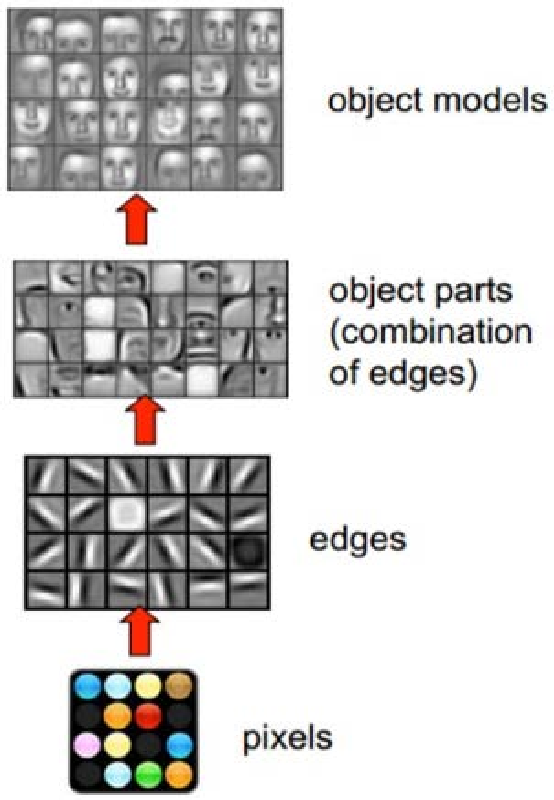
\includegraphics[width=60mm]{feat_level.pdf}
\caption{An illustration of learning feature representation by levels \cite{face}.}
\label{fig:feat_level}
\end{figure}

\begin{remark}
The layer-based learning strategy is reasonable as it is consistent with the way human used to learn things. For example, if want learn the meaning of a paragraph, we may first want to learn the meaning of each single word.
Next, with the meaning of each word and their combination in the sentences, we can learn the meaning of each sentence. Then with the meaningful of each sentence, it is much easier for us to learn the meaning of the whole paragraph.
\end{remark}

\section{Feature Learning: Models and Algorithms}

Deep neural networks or deep learning is a learning model where the deep architecture is applied to perform the intellectual learning like learning to represent features. This ability, together with the efficient learning algorithms that can ensure this ability, point out a new direction in the task of unsupervised feature learning, i.e., learning deep representation of the feature. In this section, I will review the work related to the deep learning in recent years, with a focus on some typical learning architectures and learning algorithms. The application of it in unsupervised feature learning will be discussed in the next section.


\subsection{Background and Motivation}

Deep learning methods aim at learning feature hierarchies with features from higher levels formed by the composition of features from lower levels. Learning features at multiple levels of abstraction allows a system to learn complex functions that map the input data to output feature, which is especially important for higher-level abstractions where humans often don't know how to specify the explicit feature extraction algorithms.

Deep architecture refers to the model architecture that can learn multiple levels non-linear transformation. And the depth of architecture refers to the number of levels of composition of non-linear transformation in the function learned. Most current popular learning algorithms such as Logistic Regression (no hidden layer), Support Vector Machine (one hidden layer) and Boosting (one hidden layer) are using the shallow architectures. However, inspired by the architectural depth of the brain, neural network researchers had wanted for decades to train deep multi-layer neural networks. Unfortunately, no successful attempts were reported: researchers reported positive experimental results with typically two or three levels (i.e., one or two hidden layers), but training deeper networks consistently yielded poorer results.

In 2006, a breakthrough in feature learning and deep learning was initiated by Geoff Hinton, he introduced Deep Belief Networks (DBNs) together with a learning algorithm\cite{Hinton} and was quickly followed up in the same year by many others. The central idea, referred to as \textit{greedy layerwise unsupervised pre-training}, was to learn a hierarchy of features one level at a time, using unsupervised feature learning to learn a new transformation at each level to be composed with the previously learned transformations.

Since 2006, deep networks for feature learning have been applied widely with success not only in classification tasks, but also in regression, dimensionality reduction, speech recognition, object segmentation, information retrieval, robotics, natural language processing and collaborative filtering\cite{AI}.


\subsection{Deep Belief Networks (DBNs)}

\begin{figure}[t]
\centering
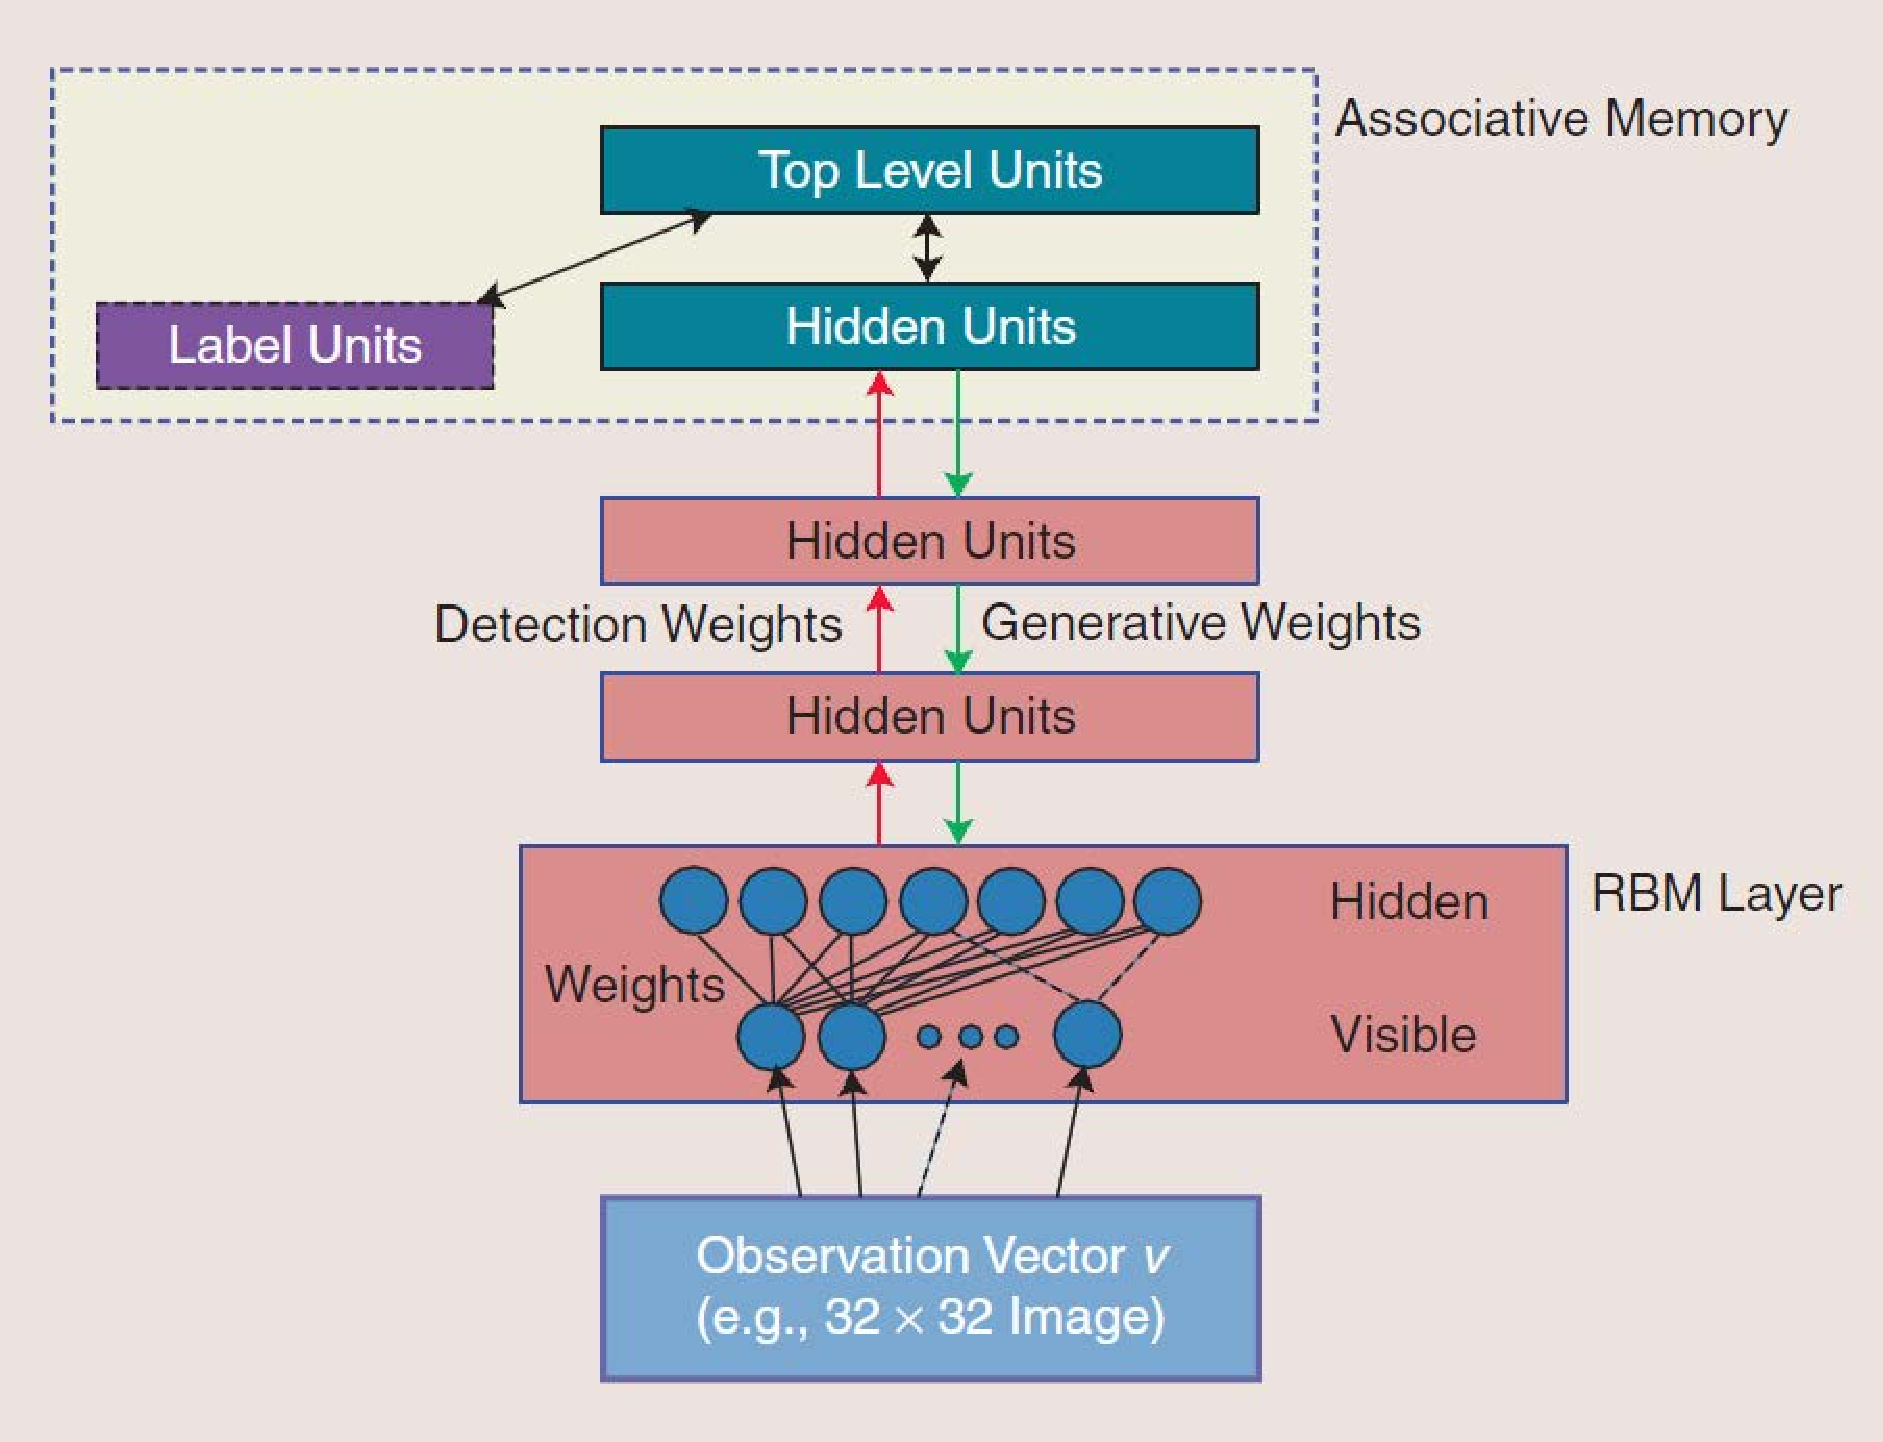
\includegraphics[width=80mm]{dbn.pdf}
\caption{Illustration of deep belief networks\cite{new_frontier}.}
\label{fig:dbn}
\end{figure}

There are several types of deep neural networks such as deep belief networks (DBNs) and convolutional neural networks (CNNs). Among them DBNs are not
only one of the milestones in the realm of deep learning, but also very capable for unsupervised feature learning. Therefore, in this part, I'll mainly focus on DBNs, and cover its details in learning feature representation.


DBNs is a hybrid model consisting of two parts. As shown in Fig. \ref{fig:dbn}, the top two levels are undirected graph model which form the associative memory, the remaining layers are directed graph model which is actually a stacked Restricted Boltzmann Machines (RBM). Different from the CNNs, DBNs is a stochastically learning architecture whose object
function depends on the learning purpose. Generally speaking, DBNs can be trained as a discriminative model or a generative model. In Fig. \ref{fig:dbn} , the discriminative model is a ``bottoms-up'' approach (red arrow), trying to
learn the detection weights via optimizing a posterior probability $P(L|O)$, where $L$ indicates the label while $O$ is the observation; the generative model is a ``top-down'' approach (green arrow), trying to learn the generative weights via optimizing a joint probability $P(L,O)$.

%The details of the learning strategies will be discussed in the next part of this section.

Another description of DBNs is from Hinton et al. \cite{Hinton}, where they showed that Restricted Boltzmann Machine (RBMs) can be stacked and trained in a greedy manner to form so-called DBNs. They model the joint distribution between observed vector $\mathbf{x}$ and the $l$ hidden layers as:
\begin{equation}
P(\mathbf{x},h^1,\ldots,h_l)=\Big(\prod_{k=1}^{l-2} P(h^k|h^{k+1})\Big)
P(h^{l-1},h^l),
\end{equation}
where $x=h^0,\ P(h^{k-1}|h^k)$ is a conditional distribution for the visible units conditioned on the hidden units of the RBM at level $k$, and $P(h^{l-1},h^l)$ is the visible-hidden joint distribution in the top-level RBM.


The greatest advantage of DBNs is its capability of learning multi-level representation of feature, which is achieved through a layer-wise training strategy where the higher-level features are learned based on the features produced by the previous layers. Therefore, the higher-level features are believed to be more complicated and can better represent the information extracted from the structure of input data. Furthermore, we can also prove that after we adding another layer of features, we improve a variational lower bound on the log probability of the training data \cite{Hinton}.



\subsection{Challenge of Training Deep Neural Networks}

After having motivated by the need for deep architecture and the advantages of deep belief networks, now we turn to the difficult problem of training them.
Experimental evidence suggests that training deep architectures is more difficult than training shallow architectures\cite{AI}.

One of the biggest problems when applying traditional gradient-based training for deep neural networks is that the random initialized multi-layer neural networks gets stuck in ``apparent local minima or plateaus'', and it becomes more difficult to obtain good generalization as the architecture gets deeper. When starting from random initialization, the solutions obtained with deeper neural networks perform even worse than the solutions obtained for networks with 1 or 2 hidden layers. This happens even though $k+1$-layer nets can easily represent what a $k$-layer net can represent, but the converse is not true.

So, to take advantages of deep architectures, we need a new way to train these models.

\subsection{Train DBNs for Feature Learning}

In this part, I'll discuss the training strategy in deep learning architecture. We will focus on the training of DBNs. To start this subsection, let's first introduce the Restricted Boltzmann Machines (RBM).

\subsubsection{Restricted Boltzmann Machines}

Boltzmann Machines (BMs) are a particular form of log-linear Markov Random Field (MRF), i.e., for which the energy function is linear in its free parameters. To make them powerful enough to represent complicated distributions (i.e., go from the limited parametric setting to a non-parametric one), we consider that some of the variables are never observed (i.e., hidden). By having more hidden variables (also called hidden units), we can increase the modeling capacity of the Boltzmann Machine (BM). RBMs further restrict BMs to those without visible-visible and hidden-hidden connections. A graphical depiction of an RBM is shown in Fig. \ref{fig:rbm}.

\begin{figure}[t]
\centering
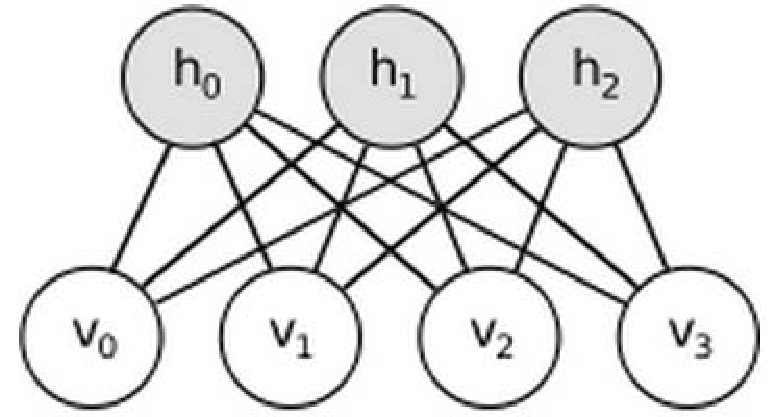
\includegraphics[width=60mm]{rbm.pdf}
\caption{A graphical depiction of an RBM.}
\label{fig:rbm}
\end{figure}

The energy function of an RBM $E(v,h)$ is defined as
\begin{equation}\label{eq:energy}
E(v,h)=-b'v-c'h-h'Wv,
\end{equation}
where W represents the weights connecting hidden and visible units and $b$ and $c$ are offsets of the visible and hidden layers respectively.
Due to the specific structure of RBMs, visible and hidden units are conditionally independent given one another. Therefore, we have
\begin{align}
  p(h|v) &=\prod_i p(h_i|v)\nonumber \\
  p(v|h) &=\prod_j p(v_j|h)
\end{align}

\subsubsection{Pre-Training}


Generally speaking, the training process of DBNs usually consists of two parts, one is the pre-training, the other is fine-tuning.

The DBN pre-training procedure treats each consecutive pair of layers in neural networks as a RBM, whose joint distribution is defined as
\begin{equation}\label{eq:distribution}
P_{\mathbf{h},\mathbf{v}}(h,v)=\frac{1}{Z_{h,v}}\cdot e^{v^TWh+v^Tb+a^Th}
\end{equation}
for the Bernoulli-Bernoulli RBM applied to binary $v$ with a second bias vector $b$ and normalization term $Z_{h,v}$, and
\begin{equation}\label{eq:distribution2}
P_{\mathbf{h},\mathbf{v}}(h,v)=\frac{1}{Z_{h,v}}\cdot e^{v^TWh+(v-b)^T(v-b)+a^Th}
\end{equation}
for the Gaussian-Bernoulli RBM applied to continuous $v$. In both cases the conditional probability $P_{h|v}(h|v)$ has the same form as that in an neural net layer.

The RBM parameters can be efficiently trained in an unsupervised fashion by maximizing the likelihood
\begin{equation}
\mathcal{L}=\prod_t \sum_h P_{h,v}(h,v(t))
\end{equation}
over training samples $v(t)$ with the approximate contrastive divergence algorithm described in \cite{rbm}, which are
\begin{align}
  \frac{\partial\log\mathcal{L}}{\partial W}&\approx \sum_t v(t)\cdot
  E_{\mathbf{h}|\mathbf{v}} \{\mathbf{h}|v(t)\}^T-\sum_t \hat{v}(t)\cdot
  E_{\mathbf{h}|\mathbf{v}} \{\mathbf{h}|v(t)\}^T \nonumber
   \\
   \frac{\partial\log\mathcal{L}}{\partial a}&\approx E_{\mathbf{h}|\mathbf{v}} \{\mathbf{h}|v(t)\}-\sum_t E_{\mathbf{h}|\mathbf{v}} \{\mathbf{h}|\hat{v}(t)\}
   \nonumber \\
   \frac{\partial\log\mathcal{L}}{\partial b}&\approx \sum_t v(t)-\sum_t \hat{v}(t)
\end{align}
with $\hat{v}(t)=\sigma(W\hat{h}(t)+b)$, where $\hat{h}(t)$ is a binary random sample from $P_{\mathbf{h}|\mathbf{v}}(\cdot|v(t))$.

To train multiple layers, one may train the first layer, freeze it,
and then use the conditional expectation of the output as the input
to the next layer and continue training next layers. Hinton and
many others have found that initializing neural network with pretrained
parameters never hurts and often helps \cite{Hinton}.

Another popular and easy-implement choice for pre-training is the greedy layer-wise unsupervised pre-training \cite{greedy}. The key idea of this approach is to learn a hierarchy of features one level at a time, using unsupervised feature learning to learn a new transformation at each level to be composed with the previously learned transformations. During the learning phase, each iteration of unsupervised feature learning adds a new layer of weights to the whole deep neural network. Finally the set of layers could be combined to transform the input data into a set of learned high-level features through a series of non-linear transformation.



\begin{remark}
If we regard the layer-wise pre-training as learning the representation of feature from the input data, then the whole pre-training process can be considered as learning the representation of the original data layer by layer. So, intuitively, learning the feature representation of data can be performed though training the deep neural networks.
\end{remark}

\subsubsection{Fine-tuning}

After pre-training, the weights between each adjacent layers can somehow reflect the relationship with the data themselves. Furthermore, in order to ensure a better performance, we use fine-tuning to adjust these weights according to different model types we assume.

For the discriminative model, back-propagation algorithm is used to adjust the detection weights by supervised learning using the labeled
data. There is nothing new about the back-propagation, the only thing we should pay attention to is that we should carefully set the learning rate since a too-big value will change the pre-trained weights a lot. However, we should also notice that there is a trade-off as a too-small value will lead to a slow tuning procedure.

For the generative model, a wake-sleep algorithm is used to tune the generative weights. Wake is a bottom-up procedure, which uses the learning RBM approach to approximate the joint distribution showed in the following term
\begin{align}
&P(v,h_1,h_2,\ldots h_n) \nonumber \\ = &P(h_1|v)P(h_2|h_1,v)\cdots
P(h_n|h_{n-1},\ldots,h_1,v).
\end{align}
Since detection weights are learned in this procedure, we can sample all the $v,h_1,h_2,\ldots,h_n$. Then, these sampled data are used to tune the generative weights, which is to maximize the following term
\begin{align}
&P(v,h_1,h_2,\ldots h_n)\nonumber \\ =& P(h_{n-1}|h_n)P(h_{n-2}|h_{n-1},h_n)\cdots P(v|h_n,\ldots h_1).
\end{align}
Since all units are known, it is easy to solve this maximization problem.
Therefore, wake stage is a ��bottom-up�� procedure tuning the generative weights. Tuning only once is not enough, so we also need the sleep stage which is similar to wake, but it is ��top-down�� approach and tunes the detection weights. We iteratively call the wake and sleep stages until the convergence is reached, which indicates the end of fine-tuning.


\section{Applications of Unsupervised Feature Learning and Deep Learning}

In the previous sections, I have shown that why we should study feature learning, what strategy we should  use in feature learning and what model we should  apply in unsupervised feature learning. In this section, I'll refer to some successful real world applications to show the powerful usage of unsupervised feature learning as well as deep learning and how these machine learning tasks benefit from the unsupervised feature learning.


\subsection{Unsupervised Feature Learning in Speech Recognition}

\begin{figure}[t]
\centering
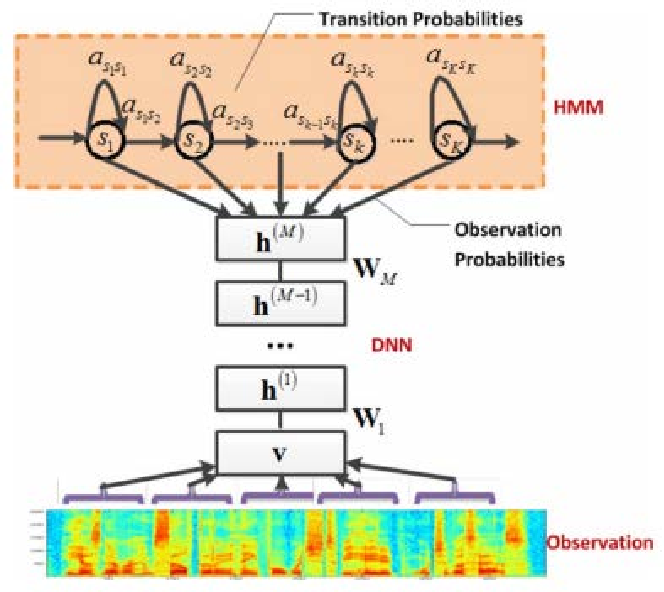
\includegraphics[width=80mm]{cd-dnn-hmm.pdf}
\caption{Diagram of the hybrid architecture in speech recognition employing a deep neural network \cite{cd-dnn-hmm}.}
\label{fig:cd-dnn-hmm}
\end{figure}

Hidden Markov models (HMMs) have been the dominant
technique for  large vocabulary speech
recognition (LVSR) for at least two decades. An HMM is a
generative model in which the observable acoustic features are
assumed to be generated from a hidden Markov process that
transitions between states $S=\{s_1,\ldots,s_K\}$. The key
parameters in the HMM are the initial state probability distribution
$\pi=\{p(q_0=s_i)\}$, where $q_t$ is the state at time $t$; the transition probability $a_{ij}=p(q_t=s_j|q_{t-1}=s_i)$; and a model to estimate the observation probabilities $p(\mathbf{x}_t|s_i)$.

Since the early 90��s, artificial neural networks (ANNs) have
been used to model the state emission probabilities of HMM
speech recognizers. While traditional Gaussian mixture
model (GMM-HMMs) models context dependency through tied
context-dependent states, ANN-HMMs were never used to do so directly.
Instead, neural networks were often factorized, e.g. into a monophone
and a context-dependent part, or hierarchically decomposed. It has been commonly assumed that hundreds or thousands of triphone states were just too many to be accurately modeled or trained within a neural network.

Only recently, Yu et al. discover
that doing so is not only feasible but works very well \cite{cd-dnn-hmm}.
As shown in Fig. \ref{fig:cd-dnn-hmm},
The foundation of the hybrid approach is the use of a
forced alignment to obtain a frame level labeling for training the
ANN. The key difference between the Context-dependent Deep-Neural-Network Hidden-Markov-Model (CD-DNN-HMM) architecture and earlier ANN-HMM hybrid architectures (and context-independent DNN-HMM) is that they apply DNN as the feature learner to extract more powerful, more robust features and model senones as the DNN output units directly.
This change offers two primary advantages. First, they can implement a CD-DNN-HMMs system with only minimal modifications to an existing CD-GMM-HMM system. Second, any improvements in modeling units
that are incorporated into the CD-GMM-HMM baseline system,
such as cross-word tri-phone models, will be accessible to the
DNN through the use of the shared training labels.

If DNNs can be trained to better predict senones, then
CD-DNN-HMMs can achieve better recognition accuracy than tri-phone GMM-HMMs. More precisely, in the CD-DNN-HMMs, the decoded word sequence $\hat{w}$ is determined as

\begin{equation}\label{eq:cd-dnn}
  \hat{w}=\arg\max_w p(w|\mathbf{x})=\arg\max_w \frac{p(\mathbf{x}|w)p(w)}{p(\mathbf{x})},
\end{equation}
where $p(w)$ is the language model probability, and
\begin{align}
  p(\mathbf{x}|w)&=\sum_{q} p(\mathbf{x},q|w)p(q|w) \\
  &\cong \max \pi(q_0) \prod_{t=1}^T a_{q_{t-1}q_t}\prod_{t=0}^T p(\mathbf{x}_t|q_t)
\end{align}
is the acoustic model probability. Note that the observation probability is
\begin{equation}
p(\mathbf{x}_t|q_t)=\frac{p(q_t|\mathbf{x}_t)p(\mathbf{x}_t)}{p(q_t)},
\end{equation}
where $p(q_t|\mathbf{x}_t)$ is the state (senone) posterior probability estimated from the DNN, $p(q_t)$ is the prior probability of each state (senone) estimated from the training set, and $p(\mathbf{x}_t)$ is independent of the word sequence and thus can be ignored.

Utilizing Hinton's DBN pre-training (unsupervised feature learning) procedure and fine-tuning, this model can lead to very promising results.
Table \ref{tab:cd-dnn} shows the comparison between the CD-GMM-HMM baseline results and the CD-DNN-HMM results \cite{Frank}.
\begin{table}[h]
\captionsetup{font={small}}
\caption{Comparison between CD-GMM-HMM Baseline Results and CD-DNN-HMM Results on Word Error Rate (WER).}
\centering
\begin{tabular}{|c|c|c|}
\hline
Acoustic Model & \#Params & WER (\%)  \\
\hline\hline
 GMM 40mix, BMMI & 29.4M & 23.6 \\ \hline
 CD-DNN 1 layer $\times$ 4634 nodes & 43.6M & 26.0 (+10\%)  \\ \hline
 + 2$\times$5 neighbor frames & 45.1M & 22.4 (-14\%)  \\ \hline
 CD-DNN 7 layers $\times$2048 nodes & 45.1M & 17.1 (-14\%)  \\ \hline
 + updated state alignment & 45.1M & 16.4 (-4\%)\\ \hline
 + sparsification 66\% & 15.2M nz & \textbf{16.1} (-2\%) \\ \hline
\end{tabular}\label{tab:cd-dnn}
\end{table}

From the table we can see that the unsupervised feature learning and deep learning can significantly improve the performance of recognition, e.g. the word error rate drops about 31\%. Also, we may notice that the effective exploitation of neighbor frames is also one of the DNN's strengths. Moreover, Fig. \ref{fig:layer} demonstrates how the sentence accuracy improves as more layers are added in the CD-DNN-HMM. When three
hidden layers were used, the accuracy increased to 69.6\%.
The accuracy further improved to 70.2\% with four hidden
layers and 70.3\% with five hidden layers. Overall, using the
five hidden-layer models provides us with a 2.2\% accuracy
improvement over the single hidden-layer system when the
same alignment is used, and probably we could expect more when more hidden layers are added.



%\begin{table*}[ht]\label{Tab:1}
%\captionsetup{font={small}}
%\caption{Standard GMM-HMM vs. CD-DNN-HMM for single-pass speaker-independent recognition on five speech-to-text test sets. Also shown are our group's best-ever GMM-HMM result for three of the test sets. Transcription word-error rates are given in $\%$.}
%\centering
%\begin{tabular}{|c|c|c|c|c|c|c|c|}
%\hline
%acoustic model \& training & recognition mode & \multicolumn{2}{c|}{RT03S}  & Hub5'00 & \multicolumn{2}{c|}{voicemails} & teleconf \\
%& & FSH & SW & SWB & MS& LDC &  \\
%\hline\hline

%GMM 40-mix, ML, SWB 309h & single-pass SI & 30.2 & 40.9 & 26.5 & 45.0 & 33.5 & 35.2 \\
%GMM 40-mix, BMMI, SWB 309h & single-pass SI & 27.4&37.6 &23.6 &42.4 &30.8 &33.9 \\
%CD-DNN 7 layers x 2048, SWB 309h & single-pass SI & 18.5&27.5 &16.1 &32.9 &22.9 &24.4 \\
%(rel. change GMM BMMI��CD-DNN) & &(-33\%) &(-27\%) &(-32\%) &(-22\%) &(-26\%) &(-28\%) \\
%\hline\hline
%GMM 72-mix, BMMI, Fisher 2000h & multi-pass adaptive &18.6 &25.2 &17.1 & & & \\
%\hline
%\end{tabular}
%\end{table*}

\subsection{Unsupervised Feature Learning in Information Retrieval}

The unsupervised feature learning for Information Retrieval (IR) is rather recent. The approaches in the literature are mostly belong to the category
of feature-based approaches. In this part, I will show an example
on deep-structured semantic modeling (DSSM) for document retrieval.

Modern search engines retrieve documents mainly by matching the keywords in documents with those in the search query.
However, lexical matching can be inaccurate due to the fact that a concept is often
expressed using different vocabularies and language styles in documents
and queries. Latent semantic models are able to map a query to its relevant documents at the semantic level where lexical-matching often
fails \cite{dssm}. These models address the language discrepancy between
Web documents and search queries by grouping different terms that
occur in a similar context into the same semantic cluster. Thus, a query
and a document, represented as two vectors in the lower-dimensional
semantic space, can still have a high similarity even if they do not share
any term. Probabilistic topic models such as probabilistic latent semantic models and latent Dirichlet allocation models have been proposed
for semantic matching to partially overcome such difficulties. However,
the improvement on IR tasks has not been as significant as originally
expected because of two main factors: (1) most state-of-the-art latent
semantic models are based on linear projection and (2) these models are often trained in an unsupervised manner using
an objective function that is only loosely coupled with the evaluation
metric for the retrieval task.

\begin{figure}[t]
\centering
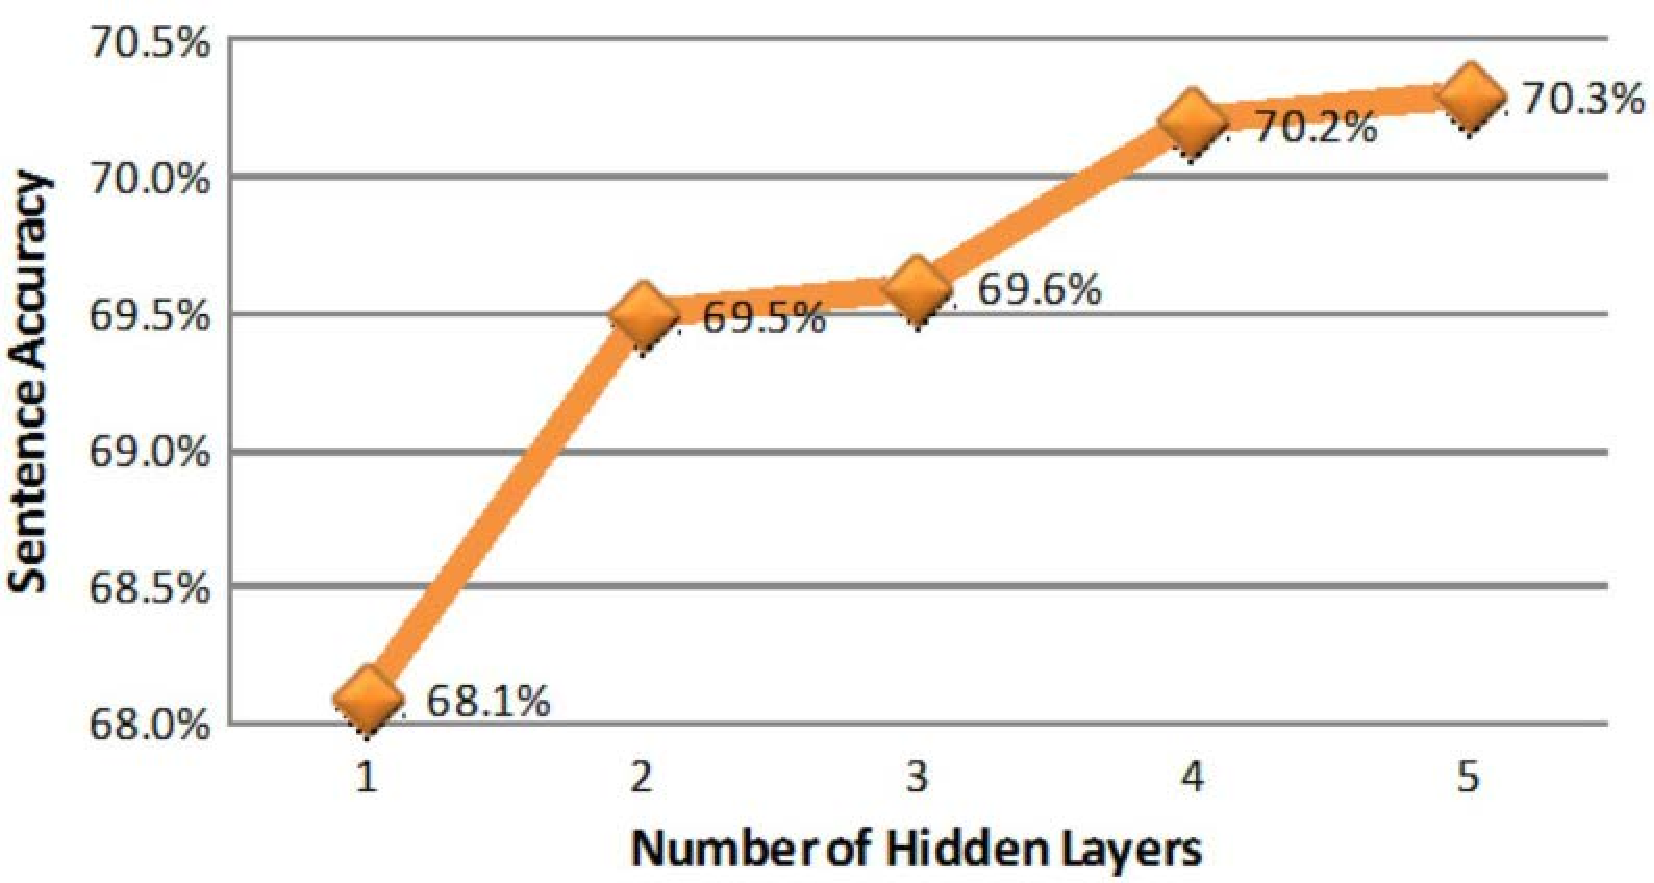
\includegraphics[width=80mm]{layer.pdf}
\caption{Sentence Accuracy versus number of hidden layers. Context-dependent models with 2K hidden units per layer were used to obtain the results \cite{cd-dnn-hmm}.}
\label{fig:layer}
\end{figure}


In order to improve semantic matching for IR, two lines of research have been conducted to extend the above latent semantic models. The first is the semantic hashing approach proposed by Salakhutdinov and Hinton \cite{hashing}, which is extended on semantic modeling using auto-encoder. They demonstrated that hierarchical semantic structure embedded
in the query and the document can be extracted via unsupervised feature learning and deep learning.
Superior performance to the conventional LSA is reported \cite{hashing}.
However, in this approach the model parameters are
optimized for the reconstruction of the documents rather than for
differentiating the relevant documents from the irrelevant ones for
a given query. As a result, the deep learning models do not
significantly outperform the baseline retrieval models based on
keyword matching.
In the second line of research, click-through data, which consists of a list
of queries and the corresponding clicked documents, is exploited for
semantic modeling so as to bridge the language discrepancy between
search queries and Web documents in recent studies \cite{click}. These
models are trained on click-through data using objectives that tailor to
the document ranking task. However, these click-through-based models
are still linear, suffering from the issue of expressiveness. As a result,
these models need to be combined with the keyword matching models
(such as BM25) in order to obtain a significantly better performance
than baselines.



The DSSM approach introduced in \cite{dssm} aims to combine the strengths of the above two lines of work while overcoming their weaknesses. It uses the DNN architecture to capture complex semantic properties of the query and the document, and to rank a set of documents for a given query. Briefly, a nonlinear projection is performed first to map the query and the documents to a common semantic space. Then,
the relevance of each document given the query is calculated as the
cosine similarity between their vectors in that semantic space.

Fig. \ref{fig:ir} demonstrates the DNN part for unsupervised feature learning in DSSM framework. The DNN is used to map high-dimensional sparse text feature into low-dimensional dense features in a semantic space. The first hidden layer, with 30k units, accomplishes word hashing. The word-hashed features are then projected through multiple layers of non-linear projections. The final layer's neural activities in this DNN form the feature in the semantic space. Let $x$ denote the input term vector, $y$ as the output vector, $l_i\ i=1,\ldots,N-1$, as the intermediate hidden layers, $W_i$ as the $i$-th projection matrix, and $b_i$ as the $i$-th bias vector, we have
\begin{align}\label{eq:dssm}
  l_1&=W_1x \nonumber \\
  l_i&=f(W_il_{i-1}+b_i),\ i>1 \nonumber \\
  y&=f(W_N l_{N-1}+b_N),
\end{align}
where \textit{tanh} function $f(x)=\frac{1-e^{-2x}}{1+e^{-2x}}$ is used for hidden units and output layer, and the semantic relevance between a query Q and a document D can then be computed as the cosine distance
\begin{equation}\label{cosine}
  R(Q,D) = cosine(y_Q,y_D)=\frac{y_Q^T y_D}{\|y_Q\|\|y_D\|},
\end{equation}
where $y_Q$ and $y_D$ are the concept vectors of the query and the document respectively.


\begin{figure}[t]
\centering
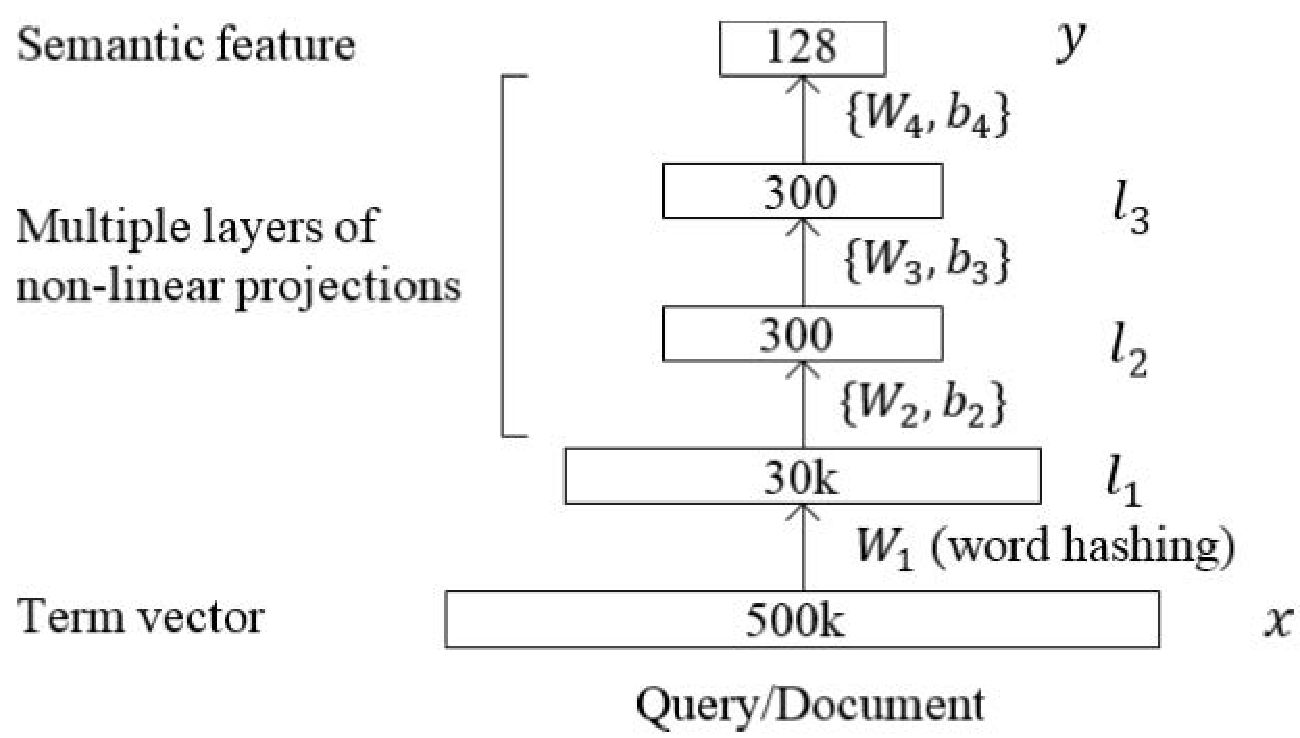
\includegraphics[width=80mm]{ir.pdf}
\caption{The DNN component of the DSSM architecture for computing semantic
features \cite{Yudong}.}
\label{fig:ir}
\end{figure}



The evaluations of the impact of using unsupervised feature learning in modeling semantic information embedded in a query and a document are shown in Table \ref{tab:dssm}.

\begin{table}[h]
\captionsetup{font={small}}
\caption{Comparative results with the previous state of the art
approaches and various settings of DSSM.}
\centering
\begin{tabular}{|c|c|c|c|c|}
\hline
No. & Models & NDCG@1 & NDCG@3  & NDCG@10 \\
\hline\hline

 1 & TF-IDF & 0.319 & 0.382 & 0.462 \\ \hline
 2 & BM25 & 0.308 & 0.373 & 0.455 \\ \hline
 3 & DAE & 0.310 & 0.377 & 0.459 \\ \hline
 \hline
 4 & DNN & 0.342 & 0.410 & 0.462 \\ \hline
 5 & L-WH linear & 0.357 & 0.422 & 0.495 \\ \hline
 6 & L-WH DNN & \textbf{0.362} & \textbf{0.425} & \textbf{0.498} \\ \hline
\end{tabular}\label{tab:dssm}
\end{table}
Row 1 (TF-IDF) and row 2 (BM25) are baseline models, row 3 (DAE) is deep auto-encoder based semantic hashing model proposed by \cite{hashing}, row 4-6 present results of different settings of DSSM. To be specific, row 4 (DNN) is a DSSM without word hashing, row 5 (L-WH linear) is the model built using letter tri-gram based word hashing (L-WH) and row 6 is the best DNN-based semantic model. The results imply that the deep structured semantic model is the best performer, beating other methods by a statistically significant margin in NDCG and demonstrating the empirical effectiveness of using DNNs and feature learning for semantic matching.

\section{Limitation}

Although unsupervised feature learning and deep learning can significant improve the performance of different machine learning tasks, there does exist some weaknesses and criticisms about them. In this section, I will give a brief introduction about some of these points.

One of the weaknesses for unsupervised feature learning and deep learning is that people do not really understand why they work. Even if we can give some intuitive explanations about the learning process, we may not be able to give a formal proof on what they learn. Another point that people often argue about the feature learning is that, unlike those manually designed features, we don't understand the learned features. This is true since neural networks take linear combination and non-linear transformation on the data, so it is hard to give a clear definition on the learned feature. The third point that people worry is about the large-scale implementation. Since we have already been in the world of big data, the unsupervised feature learning and deep learning must handle big data in order to make their own contributions.


\section{Conclusions and Future Work}


Let machine learn the feature by themselves is fascinating as well as challenging. And fortunately the unsupervised feature learning gives us a chance to make it come true. In this literature survey, a broad overview of unsupervised feature learning on different aspects is given by answering the following questions such as why we study unsupervised feature learning and deep learning, how to let machine learn feature representation by themselves, which model should we use for unsupervised feature learning and how can machine learning tasks benefit from unsupervised feature learning and deep learning. I not only show how the deep learning can be used for unsupervised feature learning, but also give some intuitions about why it works. Two real world applications on speech recognition and information retrieval have been presented to show that unsupervised feature learning can be really helpful to their tasks. Moreover, some limitations are also introduced to remind us that the area of unsupervised feature learning and deep learning still need to be further explored.

For the future of this work, the task of feature learning will not be restricted to unsupervised method, I will investigate some supervised approaches to learn better feature representations. Besides, I will also explore more feature learning models like sparse auto-encoder and convolution neural network. Both of them are wildly used as DBN and have significant impact on their corresponding areas. Finally, since feature learning still has some limitations, I would like to make some efforts to find the latest progress on solving those problems.

\section*{Acknowledgement}

I would like to thank Zi Yang for his careful review on this literature survey and many insightful comments. I would also like to thank Prof. Eric Nyberg for his advice on my presentation and his constructive suggestions on this literature survey.


\balance
\begin{thebibliography}{99}

\bibitem{review} Y. Bengio, A. Courville, and P. Vincent, ``Representation Learning: A Review and New Perspectives,'' in \textit{IEEE Trans. Pattern Analysis and Machine Intelligence}, vol. 35, no. 8, pp. 1798--1828, 2013.


\bibitem{visual} T. Serre, G. Kreiman, M. Kouh, C. Cadieu, U. Knoblich, and T. Poggio, ``A quantitative theory of immediate visual recognition,'' \textit{Progress in Brain Research, Computational Neuroscience: Theoretical Insights into Brain Function}, vol. 165, pp. 33--56, 2007.


\bibitem{face} H. Lee, R. Grosse, R. Ranganath, and A. Y. Ng, ``Unsupervised Learning of Hierarchical Representations with Convolutional Deep Belief Networks'' \textit{Communications of the ACM}, vol. 54, no. 10, pp. 95--p103, 2011.


\bibitem{new_frontier} I. Arel, D. C. Rose, and T. P. Karnowski, ``Research frontier: Deep machine learning-a new frontier in artificial intelligence research,'' \textit{Comp. Intell. Mag.}, vol. 5, no. 4, pp. 13--18, Nov. 2010.

\bibitem{Hinton} G. E. Hinton, S. Osindero, and Y. Teh, ``A fast learning algorithm for deep belief nets,'' \textit{Neural Computation}, 18, pp 1527--1554, 2006.

\bibitem{AI} Y. Bengio, ``Learning deep architectures for AI,'' \textit{Foundations and Trends in Machine Learning}, vol 2, pp 1--127. Also published as a book. Now Publisher, 2009.

\bibitem{rbm} G. Hinton, ``A Practical Guide to Training Restricted Boltzmann
Machines'', \textit{Technical Report UTML TR 2010�C003}, University of
Toronto, 2010.

\bibitem{greedy}  Y. Bengio, P. Lamblin, D. Popovici, and H. Larochelle, ``Greedy Layer-Wise Training of Deep Networks,'' \textit{Proc. Neural Information and Processing Systems}, 2006.

\bibitem{cd-dnn-hmm} G. E. Dahl, D. Yu, L. Deng, and A. Acero. ``Context-Dependent Pre-Trained Deep Neural Networks for Large-Vocabulary Speech Recognition,'' \textit{IEEE Transactions on Audio, Speech and Language Processing}, vol. 20, no. 1, Jan. 2012.


\bibitem{Frank} F. Seide, G. Li, and D. Yu, ``Conversational Speech Transcription Using Context-Dependent Deep Neural Networks'' \textit{Interspeech}, 2011.

\bibitem{dssm} P. Huang, X. He, J. Gao, L. Deng, A. Acero, and L. Heck, ``Learning deep structured semantic models for web search using clickthrough data,'' \textit{Association for Computing Machinery (ACM) International Conference Information and Knowledge Management (CIKM)}, 2013.

\bibitem{hashing} R. Salakhutdinov and G. Hinton. ``Semantic hashing,'' In \textit{Proceedings of
    Special Interest Group on Information Retrieval (SIGIR) Workshop on
    Information Retrieval and Applications of Graphical Models.} 2007.

\bibitem{click} J. Gao, K. Toutanova, and W.-T. Yih, ``Clickthrough-based latent semantic models for web search,'' In \textit{Proceedings of Special Interest Group on
Information Retrieval (SIGIR)}. 2011.


\bibitem{Yudong} L. Deng and D. Yu ``DEEP LEARNING: Methods and Applications,'' NOW Publishers, 2014.



\end{thebibliography}








\end{document}
